% classes
\documentclass{article}

% packages
\usepackage{graphicx}
\usepackage{fancyhdr} % Required for custom headers
\usepackage{lastpage} % Required to determine the last page for the footer
\usepackage{extramarks} % Required for headers and footers
\usepackage{courier} % Required for the courier font

\usepackage{color}
\usepackage{enumitem}

\usepackage{hyperref}



% page layout

\topmargin=-0.45in
\evensidemargin=0in
\oddsidemargin=0in

\textwidth=6.5in
\textheight=9.0in

\headsep=0.25in

\linespread{1.1} % Line spacing
 
\pagestyle{fancy}

% headers and footers

\fancyhf{}

\lhead{INTR 100 Breaking Intuition}

\rhead{
\includegraphics[width=0.045\textwidth]{wmlogo.jpg}}

\cfoot{Page \thepage}

% document body

\begin{document}

\vspace*{.01mm}

\begin{center}

\Large{\textcolor{blue}{\textbf{Lab 5.}  Reimagining New York City}}

\vspace{4mm}

\textit{Due by noon on Friday, November 13th}\\

\end{center}

\begin{figure}[h!]
\begin{center}
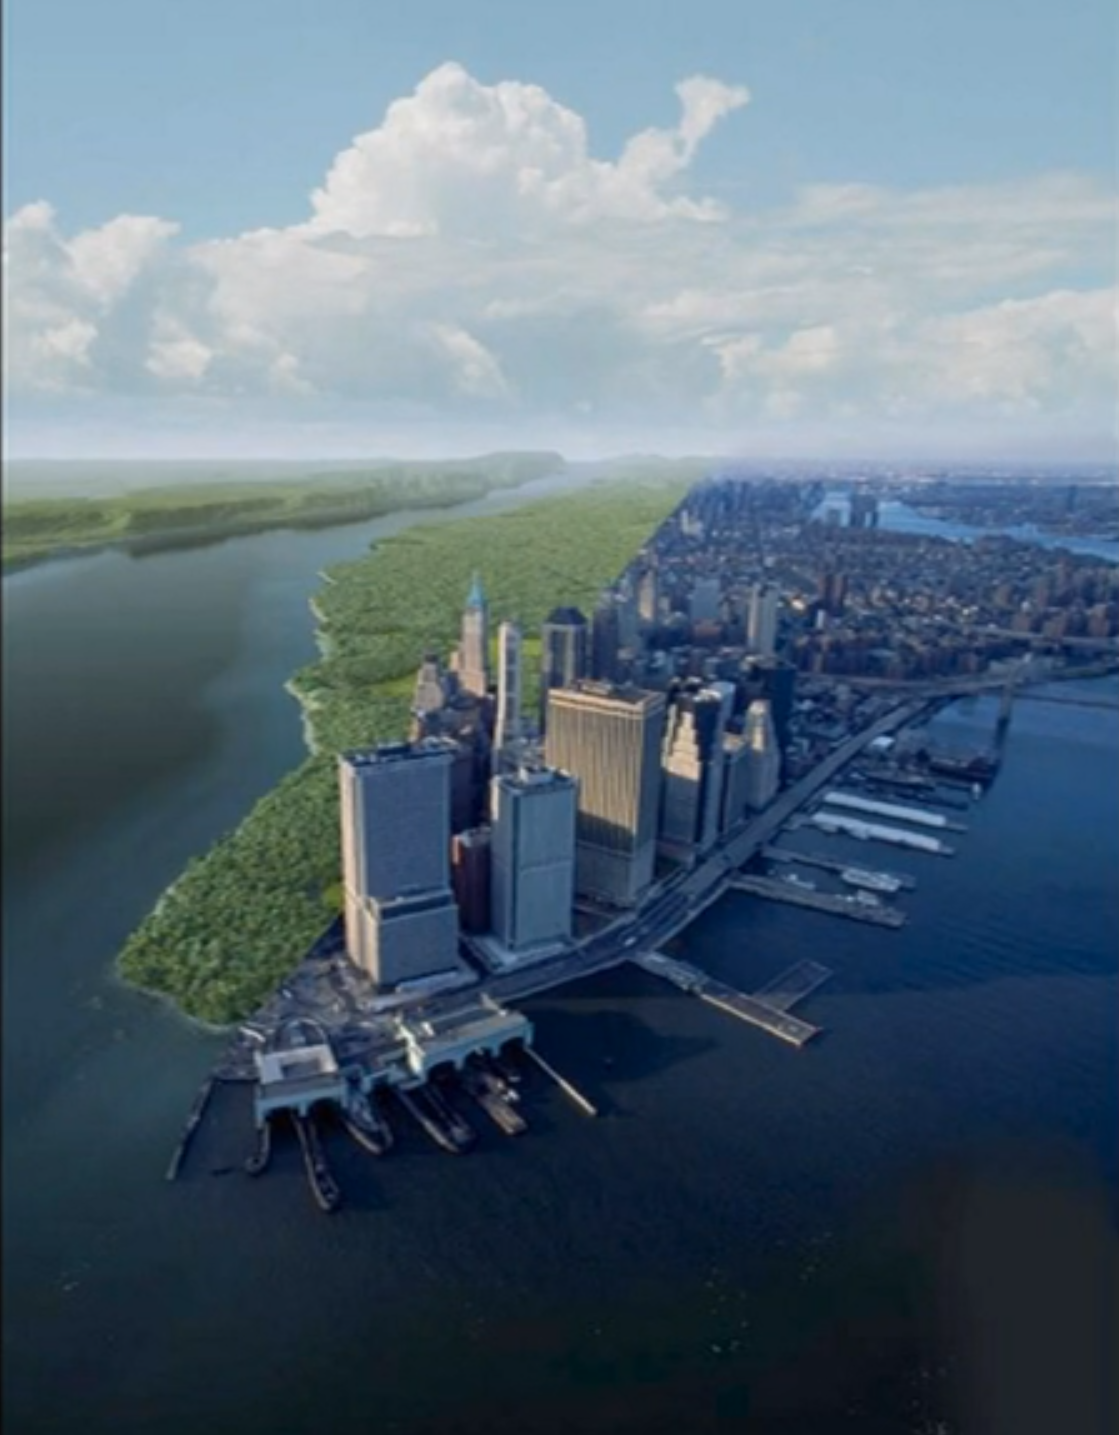
\includegraphics[width=0.75\textwidth]{nyc.png}

\end{center}
\end{figure}

\setlength{\parindent}{0cm}

\large{\textit{"And as the moon rose higher the inessential houses began to melt away until gradually I became aware of the old island here that flowered once for Dutch sailors' eyes - a fresh, green breast of the new world."}
\begin{flushright}
from Chapter 9 of F. Scott Fitzgerald's, The Great Gatsby
\end{flushright}
}


\newpage

% Enumerate the Laboratory Objectives

\large{\textbf{Laboratory in Brief:}}

\vspace{4mm}

\setlength{\leftskip}{1cm}

\setlength{\parindent}{0cm}

The purpose of this laboratory is to use the online land use planning tool Visionmaker to create a potential future for a neighborhood located somewhere in New York City.  First, you will choose a place in New York City, consider that place's natural habitat in 1609 and compare it to its existing condition in 2010.  Next, you will use Visionmaker  to reimagine transforming the existing state of your chosen place three times with an emphasis on economic, social and environmental values.  Finally, you will create a hypothetical vision for your neighborhood that optimizes environmental performance while also taking into consideration constraints for population growth and build out cost.

\vspace{4mm}

\setlength{\leftskip}{0cm}

\large{\textbf{Goals of this Laboratory:}}

\begin{enumerate}[leftmargin=15mm]

\item To choose a neighbourhood in New York City and reimagine it based on four different scenarios, each one emphasising economic, social or environmental values.

\item To reimagine that same neighbourhood while optimising environmental performance while also taking into consideration population and cost constraints.

\item To create a document that describes the vision for the chosen neighbourhood.

\end{enumerate}

% Enumerate the Laboratory Resources Needed

\large{\textbf{Things to do in Preparation for this Lab:}}

\begin{enumerate}[leftmargin=15mm]

\item Goto to the New York City Vision maker website, create an account and login.  The website may have compatibility issues with some web browsers; use Firefox or Google Chrome if you experience problems. \\ 
\url{https://visionmaker.us/nyc/}

\item Watch Eric Sanderson's June 2009 TED talk: New York - before the City \\  
\url{http://www.ted.com/talks/eric_sanderson_pictures_new_york_before_the_city}

\item Familiarise yourself with material available at the project website \\ 
\url{https://welikia.org}

\end{enumerate}

% Step by Step Instructions for Day 1

\large{\textbf{Session 1: Monday, November 2nd}}

\vspace{4mm}
\setlength{\leftskip}{1cm}
\textit{Step by Step Instructions:}

\begin{enumerate}[leftmargin=15mm]

\item Once you have created your account and logged into the Visionmaker portal, choose \textbf{Create New Vision} 
\includegraphics[width=0.25\textwidth]{create_vision.png} and set up your new vision by giving it a name.  Under the \textbf{Base on} selection button, choose \textbf{New York City (2014)} as the basis for your new vision [NOTE: ADD FIGURE].  After creating your new vision, you will want to start by choosing a neighbourhood somewhere in New York City.  If you are familiar with New York City, then this will likely be simple for you.  If you are not familiar with New York City, then try to think of some famous locations in NYC that come to your mind and consider those places.  Following are some suggested locations.

\begin{figure}[t!]
\begin{center}
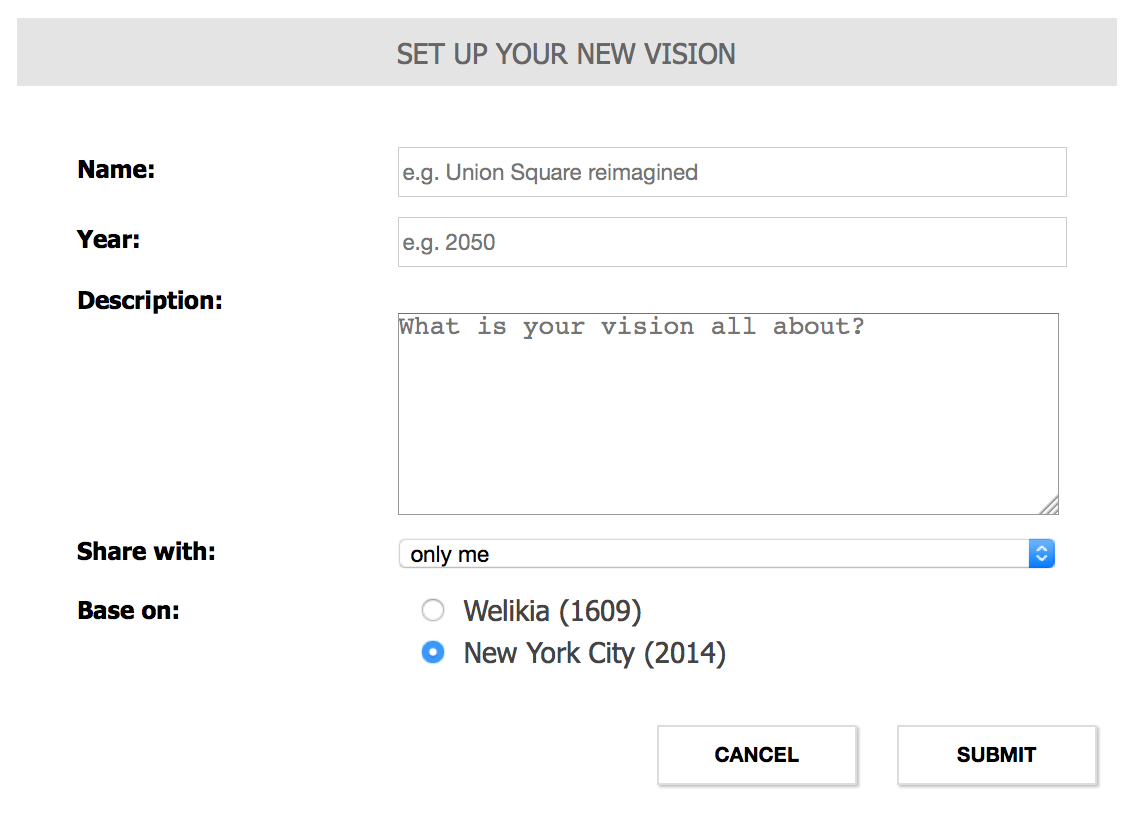
\includegraphics[width=0.75\textwidth]{vision_setup.png}
\end{center}
\end{figure}

\begin{itemize}

\item Times Square
\item The Empire State Building
\item The Brooklyn Bridge
\item Central Park
\item Broadway
\item Wall Street
\item Yankee Stadium
\item Harlem
\item Rockefeller Center
\item Madison Square Garden
\item JFK Airport

\end{itemize}

Once you have chosen your neighbourhood, find it in the Visionmaker portal and zoom in towards that location.  If you have problems finding it using the Visionmaker portal then use google to search your New York City neighborhood and then google maps to find the exact location; then use this as a guide to find your place of interest in the Visionmaker portal.  On the right hand side of the Visionmaker portal is the \textbf{zoom tool} 
\includegraphics[width=0.055\textwidth]{zoom_tool.png}, use it to bring your neighbourhood into focus at \textbf{zoom level 17}.  Explore and become familiar with your neighbourhood.

\item Once you have zoomed into your neighbourhood, click on the \textbf{Specify Vision Extent} 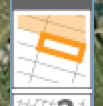
\includegraphics[width=0.055\textwidth]{vision_extent.png} tool from the toolbar on the right side of the portal interface.  Once the tool has been activated, blocks of land will highlight as the cursor traverses the aerial photograph of your New York City neighbourhood.  Use the \textbf{Specify Vision Extent} to select several continuous blocks of parcels.  Starting out by choosing eight to twelve continuous blocks of land should be good.  Once you have selected the blocks of land that will comprise your neighborhood, click on the \textbf{Save} 
\includegraphics[width=0.3\textwidth]{save_vision.png} button on the top middle of the portal.

\item After you have saved the \textbf{Vision Extent}, your neighbourhood will be transformed into individual pixels that represent the land use 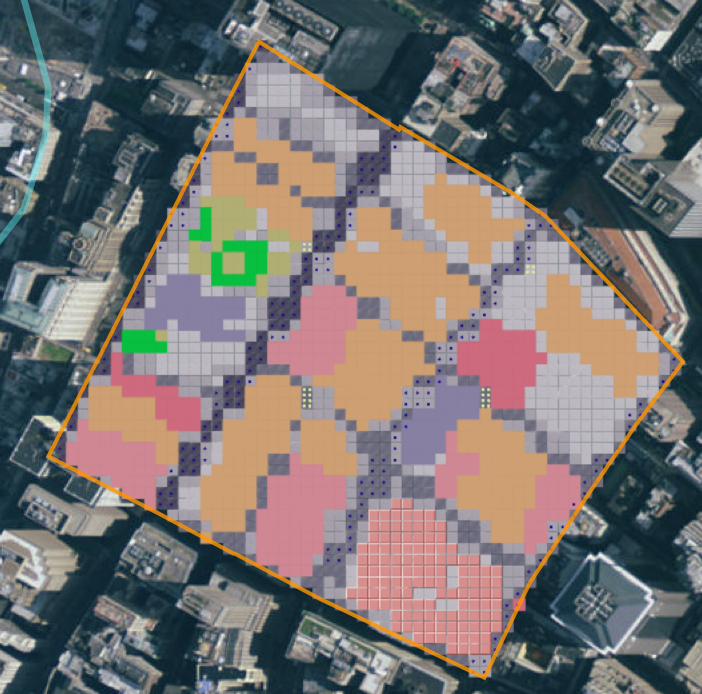
\includegraphics[width=0.2\textwidth]{pixels.png} for that location.  See the Ecosystem Tool Key [NOTE: ADD FIGURE] at the end of this document to review the colors representing various Built and Natural Environment land uses.  Select the \textbf{Grid Inspector Tool} 
\includegraphics[width=0.075\textwidth]{grid_inspect.png}and choose several of the grid cells within your neighborhood.  Note the existing land use designations as well as the natural habitat for several grid cells.  Then find the \textbf{Lifestyle/Climate Selectors} 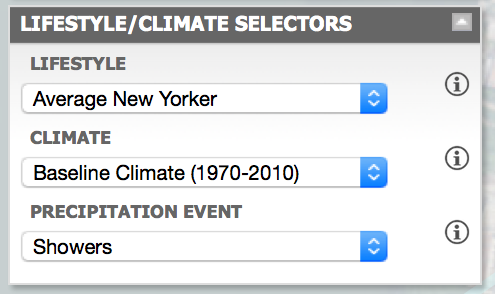
\includegraphics[width=0.25\textwidth]{lifestyle.png}toolbar and choose the lifestyle of the average person who will inhabit your neighborhood.  Next find the \textbf{Environmental Performance toolbar} 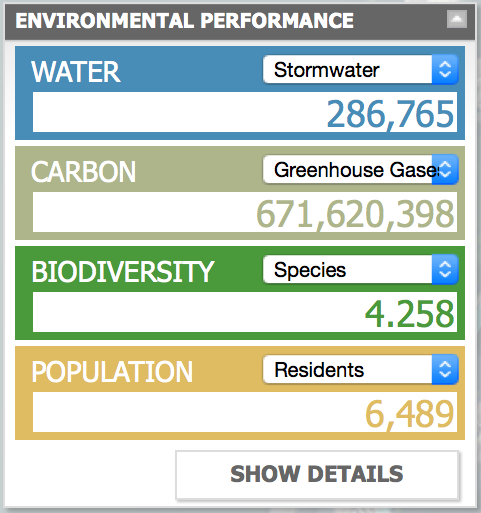
\includegraphics[width=0.3\textwidth]{env_perf.png} and choose the \textbf{Calculate button} to measure your neighborhood's environmental performance in terms of water, carbon, biodiversity, population and economics. 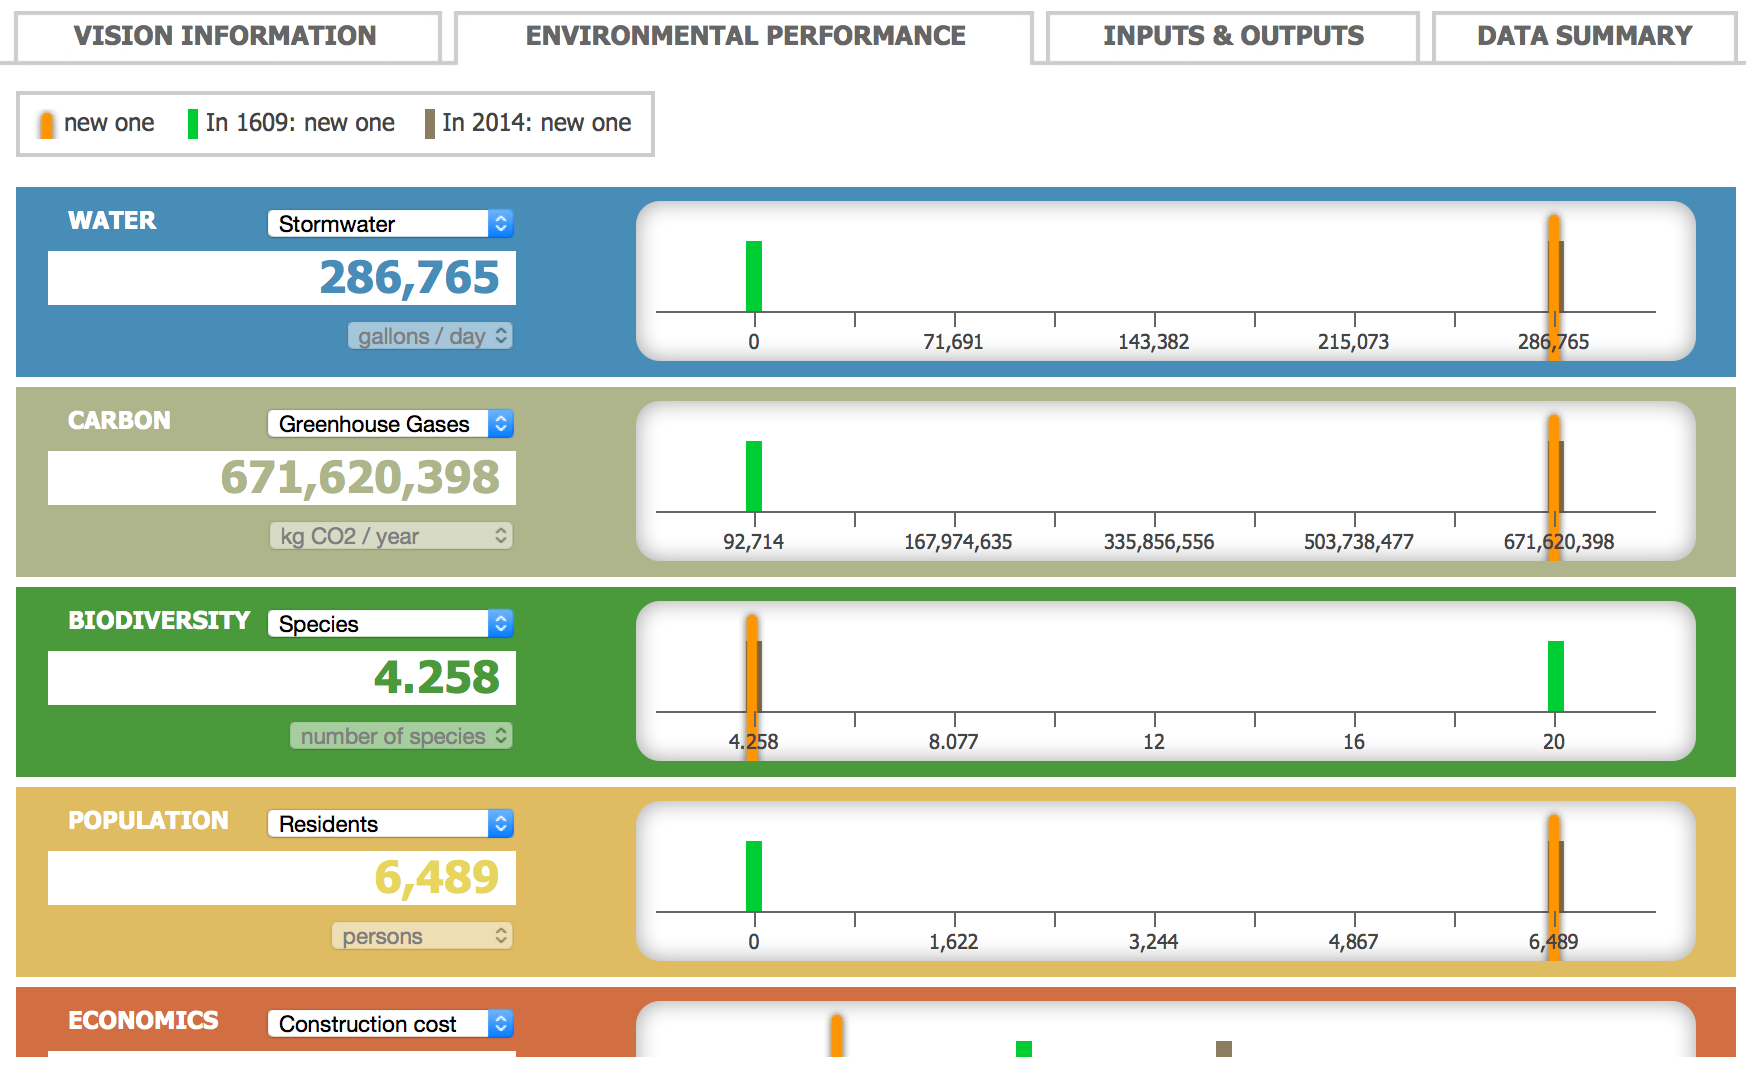
\includegraphics[width=0.35\textwidth]{env_perf2.png}  Click on the \textbf{Inputs \& Outputs bar} and also review these indicators. 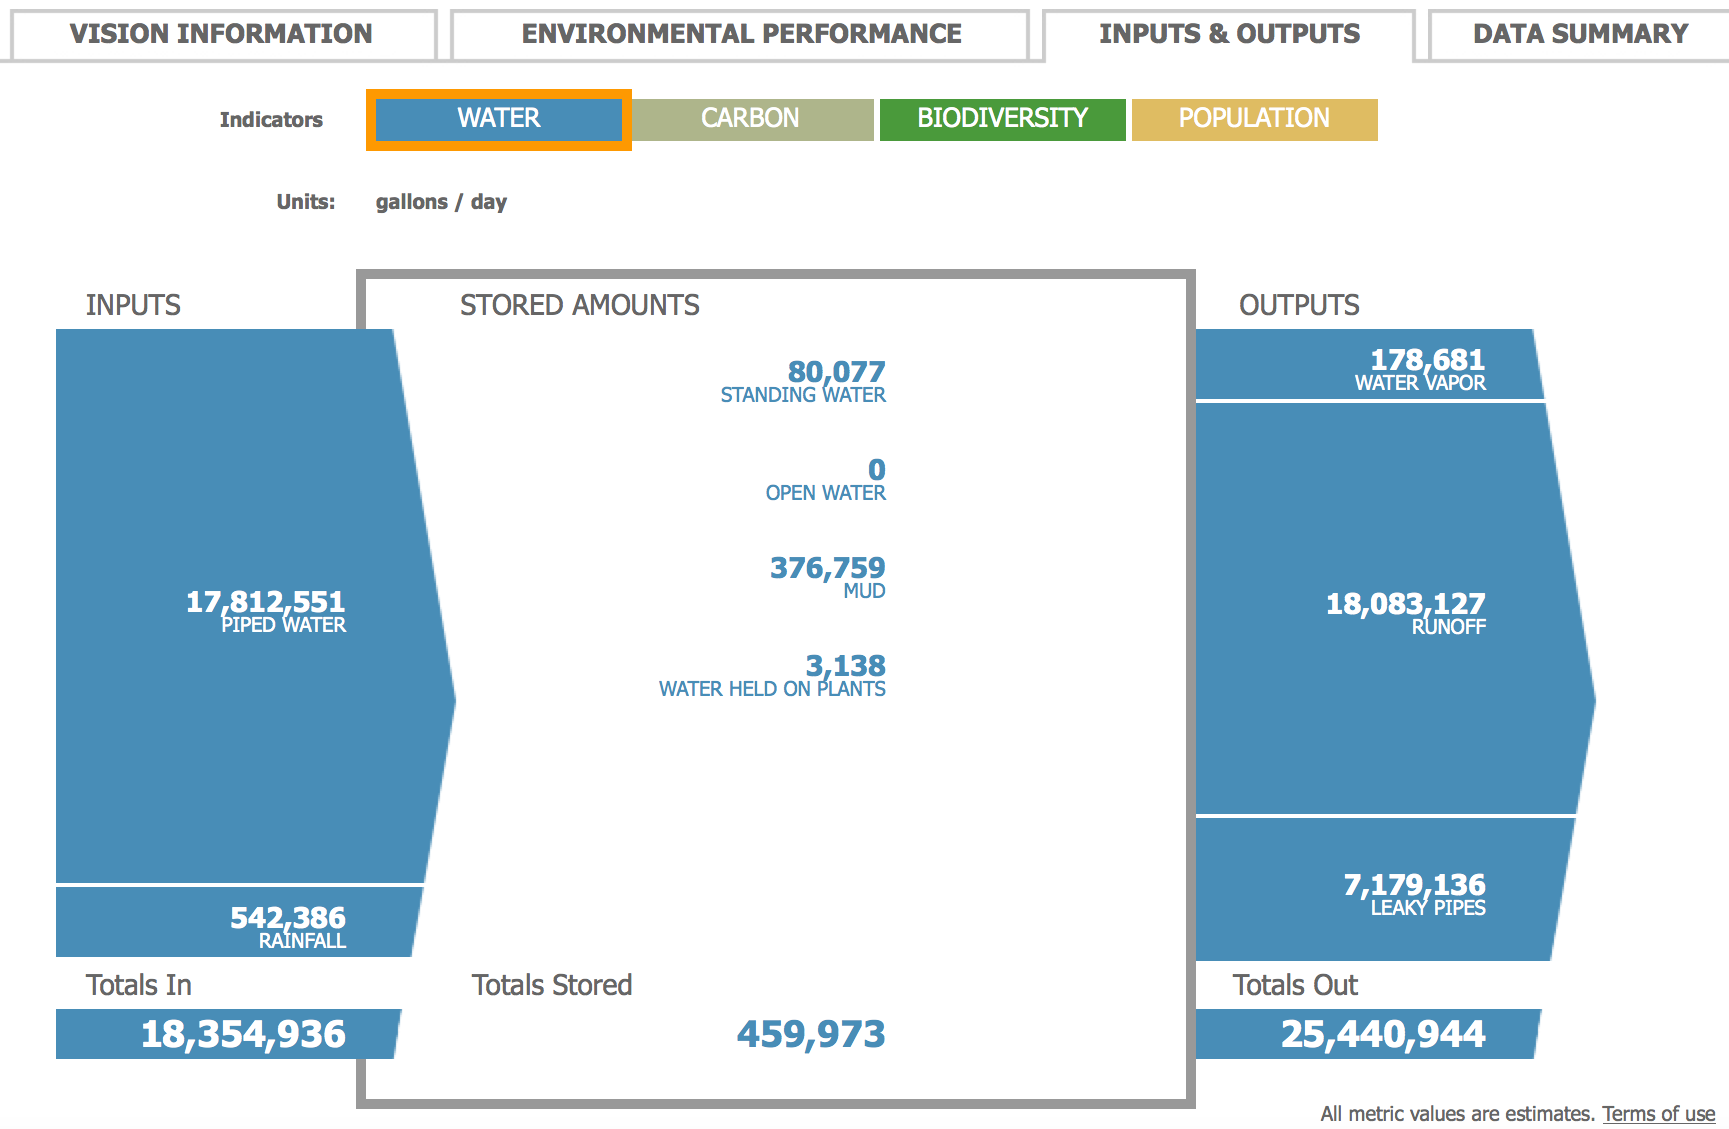
\includegraphics[width=0.35\textwidth]{in_out.png}

\item For your first exercise, pretend you are a land developer or real estate investor and build out New York City just like Donald Trump!  Find the \textbf{Buildings button} 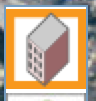
\includegraphics[width=0.075\textwidth]{buildings.png} on the right hand side of the Visionmaker portal graphical interface.  Choose one of the land uses under the buildings tab and start using that ecosystem tool 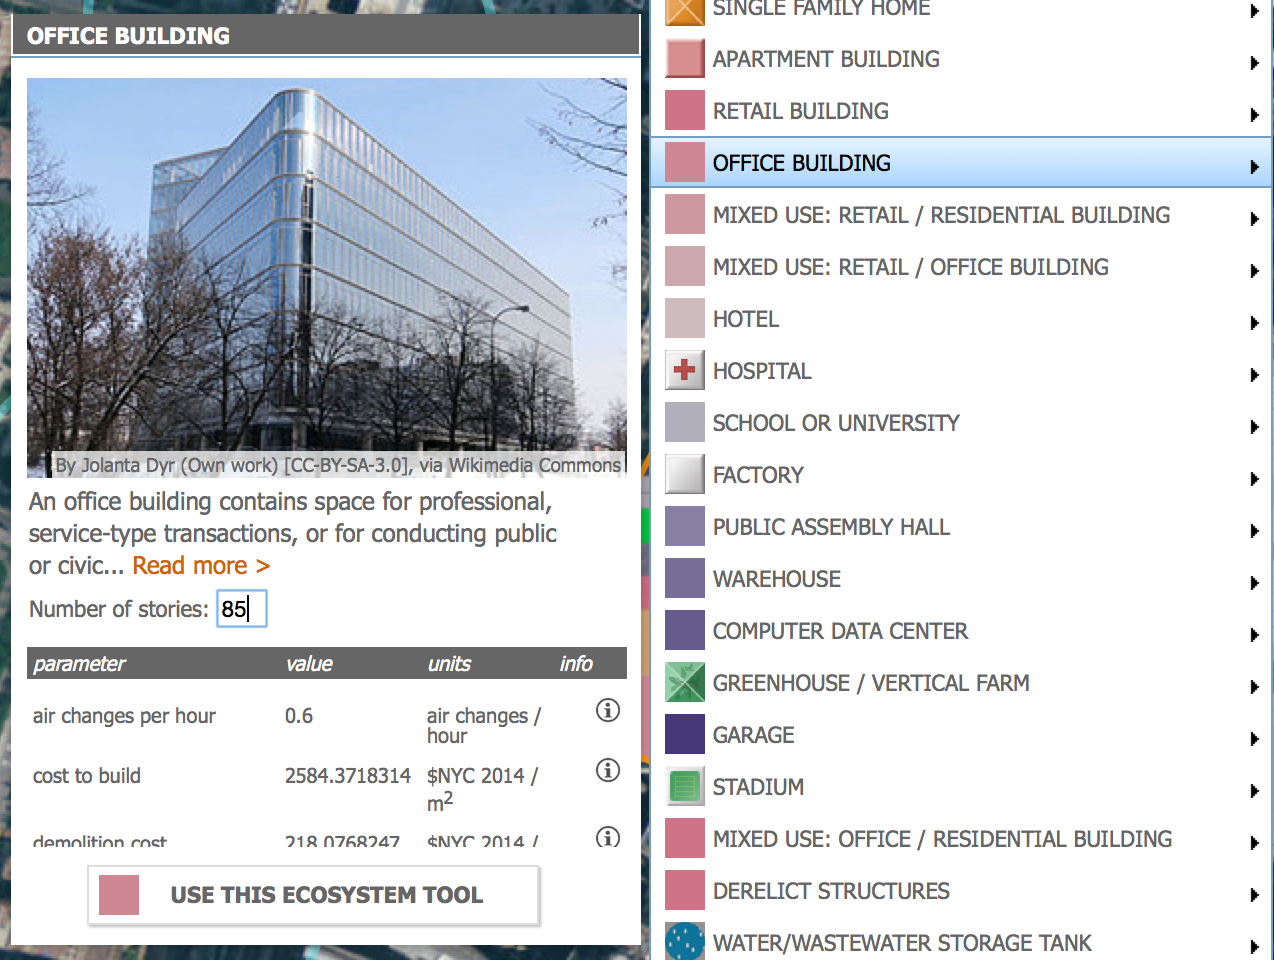
\includegraphics[width=0.45\textwidth]{office.png} to convert the existing uses to the new land use of your choice. Experiment with using the paint brush slider at the top of the page 
\includegraphics[width=0.6\textwidth]{paint_slide.png} to change the size of the ecosystem tool. \\

Imagine how to convert each grid cell in your neighbourhood into its most profitable economic use.  Transform low density residential uses to high density residential or commercial uses.  Increase the number of stories of mixed use retail and office buildings and introduce hotels (maximum number of floors is 999 although the tallest building in the world is only 160 stories).   Convert controlled access highways and freeways to parking decks, local streets and pedestrian pathways.  Add powerplants and water treatment facilities if you feel those are necessary or simply leave them external to your neighborhood vision.  Try to be realistic while also profit seeking.  \\

Once you are finished, \textbf{recalculate the environmental performance} of your neighbourhood and export the results.  A simple way to capture output for the environmental performance of your neighbourhood through the Visionmaker portal is to use the snipping tool in Windows.  This can be done by clicking the \textbf{Start} button and in the search box type \textbf{Snipping Tool} and then in the list of results, click \textbf{Snipping Tool}. 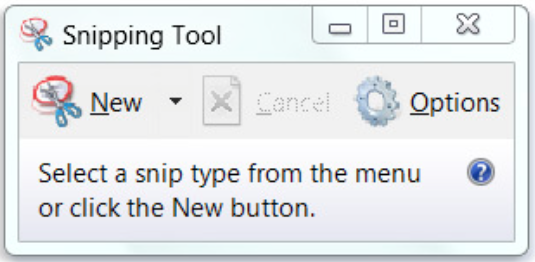
\includegraphics[width=0.35\textwidth]{snip_tool.png}

\vspace{4mm}
\setlength{\leftskip}{0cm}
\textit{Home Work 1:}

Write two or three paragraphs describing your Donald Trump scenario, describing increases in the amount of CO2 emitted and water consumed.  Compare your daytime and/or nighttime population density to another location somewhere on planet earth.  Likewise compare the construction and demolition costs to the GDP of one or more small countries.  Support your comparison and findings by using output from the environmental performance calculations.  Likewise, you can use the Snipping Tool to capture images from the web for creating figures and integrating illustrations.

\end{enumerate}

% Step by Step Instructions for Day 2

\setlength{\leftskip}{0cm}

\large{\textbf{Session 2: Wednesday, November 4th}}

\vspace{4mm}
\setlength{\leftskip}{1cm}
\textit{Step by Step Instructions:}

\begin{enumerate}[leftmargin=15mm]

\item Next imagine you are Michael Moore and transform your neighbourhood by optimising environmental and social values.  Go back to Step 4 in the Donald Trump scenario, but instead of pretending to convert land uses for maximum profit, imagine how to optimise environmental and social values.  Find the \textbf{Trees button} 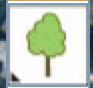
\includegraphics[width=0.075\textwidth]{trees.png} on the right hand side of the Visionmaker portal graphical interface.  Choose one of the land uses under the trees tab 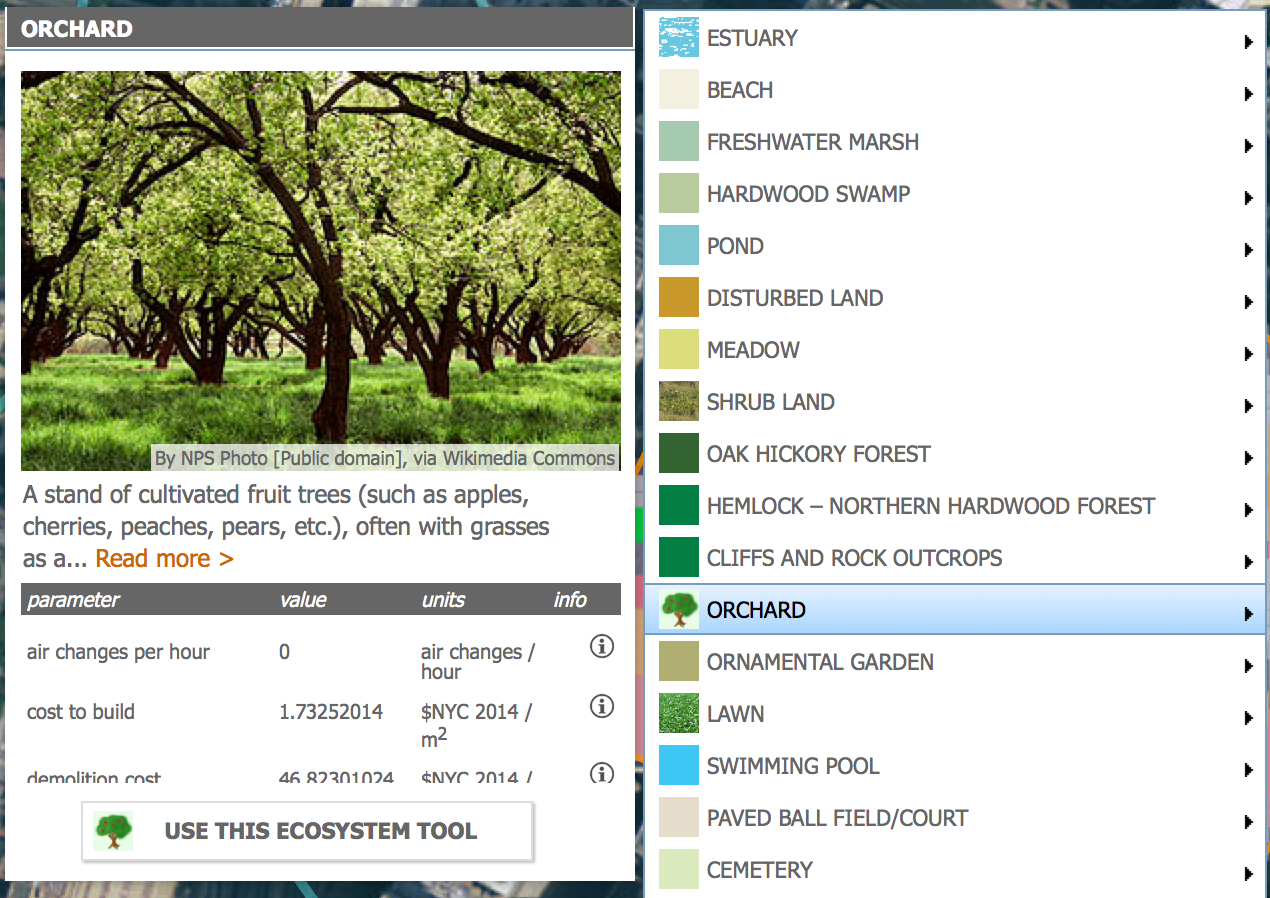
\includegraphics[width=0.4\textwidth]{trees2.png} and start using that ecosystem tool to convert the existing uses to the new land use of your choice. Once again, experiment with using the paint brush slider at the top of the page to change the size of the ecosystem tool.

Convert high density uses to natural land uses or introduce environmentally conscientious land uses such as solar energy electricity generation.  Introduce forests, orchards, public parks or community recreational facilities.  Introduce universities or public meeting spaces and reduce the functional classification of transportation facilities, introduce pedestrian pathways and other open or common spaces.  Try to reduce carbon emissions, maximise species and habitat biodiversity while also maintaining population or permitting it to increase.  

\item Once you are finished, recalculate the environmental performance of your neighborhood and export the results.  Again, a simple way to capture those results is by using the Snipping Tool as explained under Step 4 from Session 1. 


\vspace{4mm}
\setlength{\leftskip}{0cm}
\textit{Home Work 2:}

Write two or three paragraphs describing your Michael Moore scenario.  Consider the environmental performance of your transformed neighborhood in terms of stormwater and floodwater volumes.  Consider whether your post-development modifications will have a negative external impact on adjacent neighbourhoods or your particular New York City district.  How has your environmentally conscious changed Greenhouse Gas emissions?  What about species and habitat biodiversity?  As part of your modification, how many residents and workers were required to relocate?  Consider your answers to these questions and use them to construct your two to three paragraphs describing your scenario.  Feel free to compare with other locations on earth as you did with your Donald Trump scenario and likewise use figures and illustrations to support your findings.  Add this section to the output from Homework 1 and combine them into a single document that will eventually be turned in at the end of the Laboratory.

\end{enumerate}

% Step by Step Instructions for Day 3

\setlength{\leftskip}{0cm}

\large{\textbf{Session 3: Monday, November 9th}}

\vspace{4mm}
\setlength{\leftskip}{1cm}
\textit{Step by Step Instructions:}

\begin{enumerate}[leftmargin=15mm]

\item Next imagine you are New York City's Principal Land Use Planner and you need to adminster the city's Comprehensive Plan, Zoning Ordinance and Development Regulations following the Policies and Objectives set forth by the City of New York Commission and Planning Councils.  Again, go back to Step 4 in the Donald Trump scenario and follow those step-by-step instructions for transforming existing land uses, but this time you will need to meet several municipal, district and neighbourhood planning constraints.

\begin{itemize}

\item reduce greenhouse gas emissions by 15\%

\item increase species biodiversity by 15\% and habitat biodiversity by 25\%

\item maintain the existing total population

\item limit construction costs to 10 million USD

\end{itemize}

\item Once you are finished, recalculate the environmental performance of your neighbourhood and export the results.  

\vspace{4mm}
\setlength{\leftskip}{0cm}
\textit{Home Work 3:}

Write two pages describing how you achieved meeting these planning constraints for your neighbourhood.  Provide details regarding which land use conversions worked and which ones were problematic.  Give your assessment as to whether you find the Planning Constraints to be reasonable.  Return to the Snipping Tool to capture output from the Visionmaker portal and integrate them as figures and illustrations to support your work and conclusions.  Add these additional pages to the document you created from Homeworks 1 \& 2.  

\end{enumerate}
 
% Step by Step Instructions for Day 4

\setlength{\leftskip}{0cm}
 
\large{\textbf{Session 4: Wednesday, November 11th}}

\vspace{4mm}
\setlength{\leftskip}{1cm}
\textit{Step by Step Instructions:}

\begin{enumerate}[leftmargin=15mm]

\item For your final scenario pretend you are Henry David Thoreau and create a Utopian vision for your neighborhood.  When creating your vision start with the Welikia (1609) instead of the New York City (2014).  Again go back to Step 4 from Session 1 and follow those steps in order to create your ideal neighborhood from the natural environment that existing prior to the colonialization of New York.

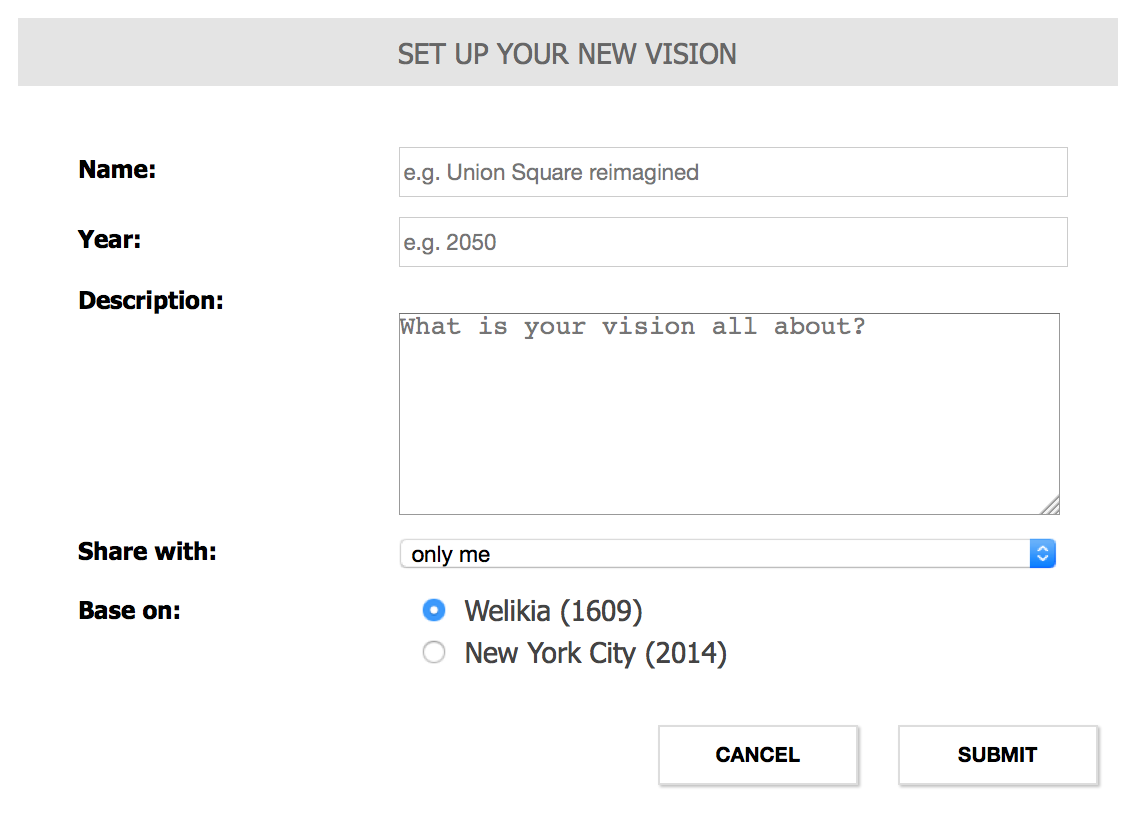
\includegraphics[width=0.5\textwidth]{old_nyc.png}

\item Once you are finished, recalculate the environmental performance of your neighbourhood and export the results.

\item Write one page describing your Utopian vision for your chosen location.  Return to the Snipping Tool to capture output from the Visionmaker portal and integrate them as figures and illustrations to support your work and conclusions.  Add this additional page to the document you created from Homeworks 1, 2 \& 3.

\end{enumerate}

% Final Output from Laboratory

\setlength{\leftskip}{0cm}

\large{\textbf{Final Output for Submittal}}

\vspace{4mm}
\setlength{\leftskip}{1cm}
\textit{Due by noon on Friday, November 13th:}
\vspace{2mm}

Finally, revisit the document you have been constructing during each of the Laboratory Sessions.  Be certain you have unified your text, figures and illustrations you created from each of the 4 Laboratories into a single document. Revise, edit and expand upon the text from your homework to create a Final Laboratory report.  Make certain the Final Report meets the following criteria.

\begin{itemize}

\item Single spaced with block paragraph style and 10 to 12 font, preferably New Times Roman, Arial, Courier or a similar font.
\item 6 to 8 pages in length
\item 1 page for the Donald Trump Scenario
\item 1 page for the Michael Moore Scenario
\item 2-3 pages for the New York City Principal Planner Scenario
\item 1-2 pages for the Henry David Thoreau Scenio
\item A section dedicated to comparison and analysis of all four scenarios
\item A conclusion

\end{itemize}

% Grading

\setlength{\leftskip}{0cm}

\textbf{Grading}

\vspace{4mm}

\setlength{\leftskip}{1cm}

\setlength{\parindent}{0cm}

This lab will be graded based on your Final Laborartory Report.  The laboratory report should include the following elements.

\newpage

\begin{center}
\begin{figure}[t!]
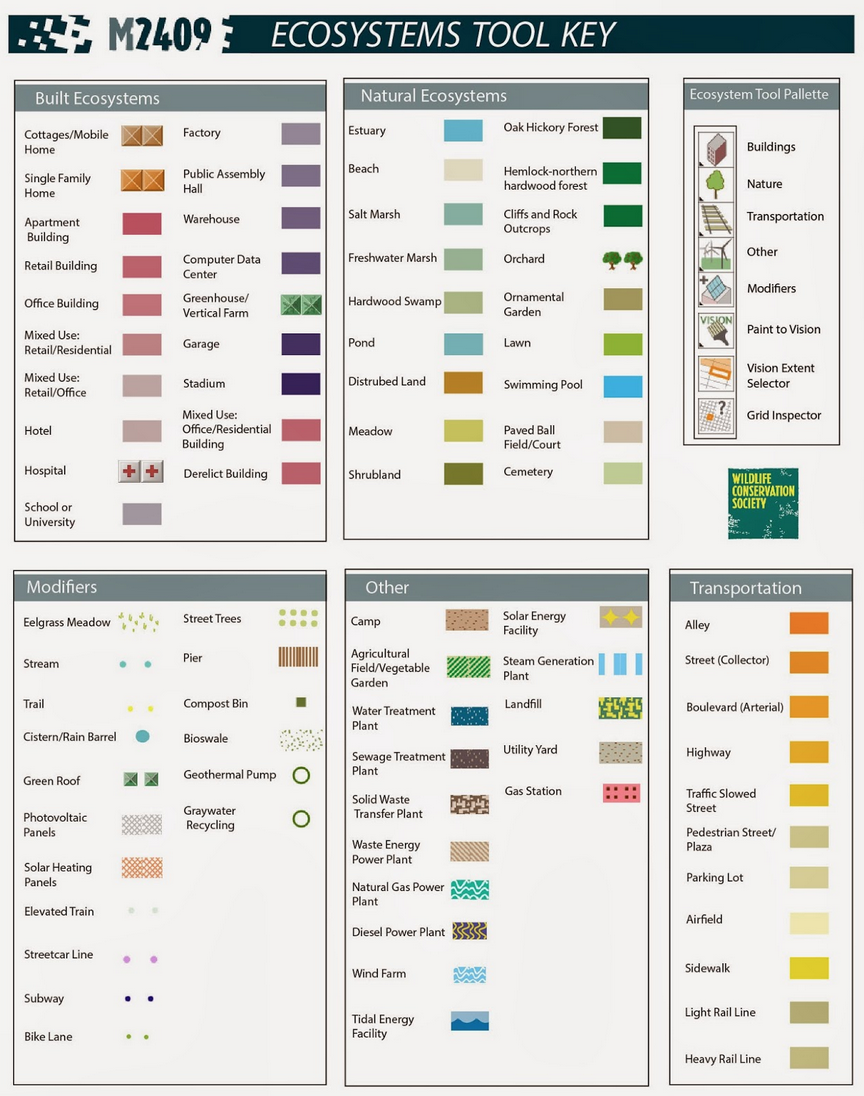
\includegraphics[width=0.9\textwidth]{key.png}
\end{figure}
\end{center}

%----------------------------------------------------------------------------------------

\end{document}